\documentclass[11pt]{article}
\usepackage[utf8]{inputenc}
\usepackage[T1]{fontenc}
\usepackage{graphicx}
\usepackage[export]{adjustbox}
\graphicspath{ {./images/} }

\begin{document}
\section*{Reading}
Alternative Investments by Inclusion

Another method of identifying alternative investments is to define explicitly which investments are considered to be alternative. In this course, we classify four types of alternative investments:

\begin{enumerate}
  \item Real assets (including natural resources, commodities, real estate, infrastructure, and intellectual property)

  \item Hedge funds (including managed futures)

  \item Private equity and private credit

  \item Structured products (including credit derivatives)

\end{enumerate}

These four categories correspond to Topics 2 to 5 of this course. Our list is not an exhaustive list of all alternative investments, especially because the CAIA curriculum is focused on institutional-quality investments. Furthermore, some of the investments on the list can be classified as traditional investments rather than alternative investments. For example, real estate and especially real estate investment trusts are frequently viewed as being traditional institutional-quality investments. Nevertheless, this list includes most institutional-quality investments that are currently commonly viewed as alternative. The next exhibit, Major Alternative Investment Fund Categories, 2021, illustrates the relative proportion of these four categories of alternative investments.\\
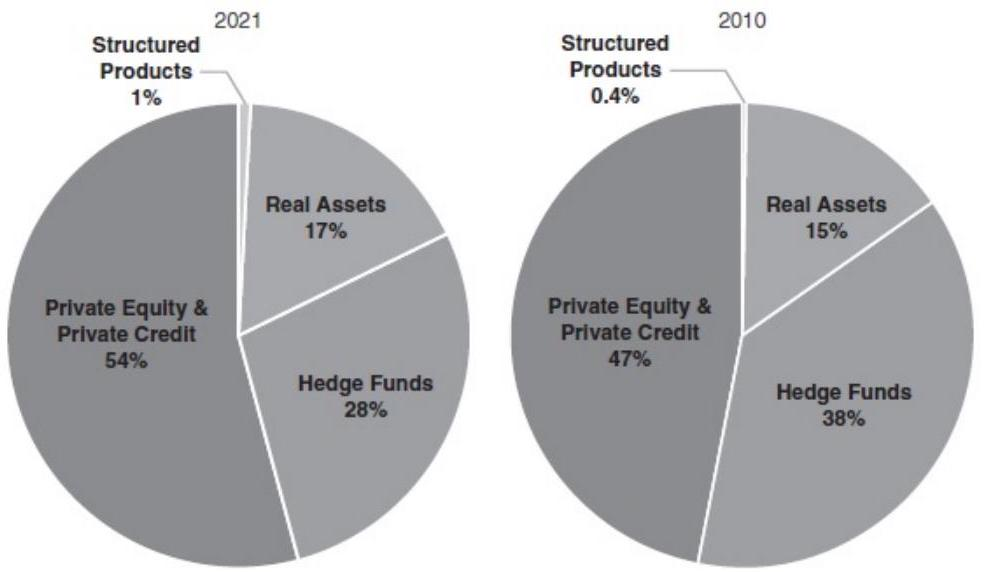
\includegraphics[max width=\textwidth, center]{2024_04_10_d2fcf76e99549155a577g-2}

Major Alternative Investment Fund Categories (percentages approximate), 2021

Source: HFR, Preqin, Willis Towers Watson

Note: These are estimates for assets under management in funds and funds of funds, and do not include direct investments.

The following sections provide brief introductions to the four categories.

\section*{Real Assets}
Real assets are investments in which the underlying assets involve direct ownership of nonfinancial assets rather than ownership through financial assets, such as the securities of manufacturing or service enterprises. Real assets tend to represent more direct claims on consumption than do common stocks, and they tend to do so with less reliance on factors that create value in a company, such as intangible assets and managerial skill. So while a corporation such as Google holds real estate and other real assets, the value to its common stock is highly reliant on perceptions of the ability of the firm's management to oversee creation and sales of its goods and services. An aspect that distinguishes types of real assets is the extent to which the ownership of the real assets involves operational aspects, such as day-to-day management decisions that have substantial impacts on the performance of the assets. For example, in many instances, direct ownership of oil reserves or stockpiles of copper involve substantially less day-to-day managerial attention than does direct ownership of real estate, infrastructure, or intellectual property.

Natural resources focus on direct ownership of real assets that have received little or no alteration by humans, such as mineral and energy rights or reserves. Commodities are differentiated from natural resources by their emphasis on having been extracted or produced. Commodities are homogeneous goods available in large quantities, such as energy products, agricultural products, metals, and building materials. Most of the investments covered in the commodities section of the CAIA curriculum involve futures contracts, so understanding futures contracts is an important part of understanding commodities. Futures contracts are regulated distinctly and have well-defined economic characteristics. For example, the analysis of futures contracts typically emphasizes notional amounts rather than the amount of money posted as collateral or margin to acquire positions.

Commodities as an investment class refer to investment products with somewhat passive (i.e., buy-and-hold) exposure to commodity prices. This exposure can be obtained through futures contracts, physical commodities, natural resource companies, and exchange-traded funds.

Some real assets are operationally focused. For the purposes of the CAIA curriculum, operationally focused real assets include real estate, land, infrastructure, and intellectual property. The performance of these types of real assets is substantially affected by the skill and success of regular and relatively frequent managerial decision-making. Traditional common stocks are typically even more highly operationally focused.

Real estate focuses on land and improvements that are permanently affixed, like buildings. Real estate was a significant asset class long before stocks and bonds became important. Prior to the Industrial Age, land was the single most valuable asset class. Only a century ago, real estate was the most valuable asset of most individuals, because ownership of a primary residence was more common than ownership of financial investments.

Land comprises a variety of forms, including undeveloped land, timberland, and farmland. Although undeveloped land might appear to belong under the category of natural resources rather than operationally focused real assets, the option to develop land often requires substantial and ongoing managerial decision-making. Timberland includes both the land and the timber of forests of tree species typically used in the forest products industry. While the underlying land is a natural\\
resource, timberland requires some level of ongoing management. Finally, farmland consists of land cultivated for row crops (e.g., vegetables and grains) and permanent crops (e.g., orchards and vineyards). Farmland necessitates substantial operations and managerial decisions.

Infrastructure investments are claims on the income of toll roads, regulated utilities, ports, airports, and other real assets that are traditionally held and controlled by the public sector (i.e., various levels of government). Investable infrastructure opportunities include securities generated by the privatization of existing infrastructure or by the private creation of new infrastructure via private financing.

Finally, while some descriptions of real assets limit the category to tangible assets, we define real assets to include intangible assets, such as intellectual property (e.g., patents, copyrights, and trademarks, as well as music, film, and publishing royalties). The opposite of a real asset is a financial asset, not an intangible asset. A financial asset is not a real asset-it is a claim on cash flows, such as a share of stock or a bond. Intangible assets, such as technology, directly facilitate production, thereby creating increased value. It can be argued that intangible assets represent a very large and rapidly increasing role in the wealth of society.

\section*{Hedge Funds}
Hedge funds represent perhaps the most visible category of alternative investments. While hedge funds are often associated with particular fee structures or levels of risk taking, we define a hedge fund as a privately organized investment vehicle that uses its less regulated nature to generate investment opportunities that are substantially distinct from those offered by traditional investment vehicles, which are subject to regulations such as those restricting their use of derivatives and leverage. Hedge funds represent a wide-ranging set of vehicles that are differentiated primarily by the investment strategy or strategies implemented. Managed futures funds are included as hedge funds in Topic 5.

\section*{Private Equity}
The term private equity is used in the CAIA curriculum to include both equity and debt positions that, among other things, are not publicly traded. In most cases, the debt positions contain so much risk from cash flow uncertainty that their short-term return behavior is similar to that of equity positions. In other words, the value of the debt positions in a highly leveraged company, discussed within the category of private equity, behaves much like that of the equity positions in the same firm, especially in the short run. Private equity investments emerge primarily from funding new ventures, known as venture capital; from the equity of leveraged buyouts of existing businesses; from mezzanine financing of leveraged buyouts or other ventures; and from distressed debt resulting from the decline in the health of previously healthy firms.

Venture capital refers to support via equity financing to start-up companies that do not have a sufficient size, track record, or desire to attract capital from traditional sources, such as public capital markets or lending institutions. Venture capitalists fund these high-risk, illiquid, and unproven ideas by purchasing senior equity stakes while the start-up companies are still privately held. The ultimate goal is to generate large profits primarily through the business success of the companies and their development into enterprises capable of attracting public investment capital (typically through an initial public offering, or IPO) or via their sale to other companies. In the context of investment management, venture capital is sometimes treated as a separate asset class from other types of private equity.

Leveraged buyouts (LBOs) refer to those transactions in which the equity of a publicly traded company is purchased using a small amount of investor capital and a large amount of borrowed funds in order to take the firm private. The borrowed funds are secured by the assets or cash flows of the target company. The goals can include exploiting tax advantages of debt financing, improving the operating efficiency and the profitability of the company, and ultimately taking the company public again (i.e., making an IPO of its new equity). Management buyouts and management buy-ins are types of LBOs with specific managerial changes.

Mezzanine debt derives its name from its position in the capital structure of a firm: between the senior secured debt and equity. Mezzanine debt refers to a spectrum of risky claims, including preferred stock, convertible debt, and debt that includes equity kickers (i.e., options that allow investors to benefit from any upside success in the underlying business, also called hybrid securities).

Distressed debt refers to the debt of companies that have filed or are likely to file in the near future for bankruptcy protection. Even though these securities are fixedincome securities, distressed debt is included in our discussion of private equity because the future cash flows of the securities are highly risky and highly dependent on the financial success of the distressed companies, and thus share many similarities with common stock. Private equity firms investing in distressed debt tend to take longer-term ownership positions in the companies after converting all or some portion of their debt position to equity. Some hedge funds also invest in distressed debt, but they tend to do so with a shorter-term trading orientation.

Private debt and direct lending strategies include loans made to borrowers outside of the banking system, specifically by hedge funds, private equity funds, and private credit funds. As regulations increased after the global financial crisis, banks facing stress tests and capital adequacy requirements backed away from lending, especially to non-investment-grade middle-market companies. Companies needing financing now need to approach direct lenders who are likely to make the loans easier and more quickly than banks, but at higher total interest costs.

\section*{Structured Products}
Structured products are instruments created to exhibit particular return, risk, taxation, or other attributes. These instruments generate unique cash flows as a result of partitioning the cash flows from a traditional investment or linking the returns of the structured product to one or more market values. The simplest and most common example of a structured product is the creation of debt securities and equity securities in a traditional corporation. The cash flows and risks of the corporation's assets are structured into a lower-risk fixed cash flow stream (bonds) and a higher-risk residual cash flow stream (stock). The structuring of the financing sources of a corporation creates option-like characteristics for the resulting securities.

Collateralized debt obligations (CDOs) and similar instruments are among the best-known types of structured products. CDOs partition the actual or synthetic returns from a portfolio of assets (the collateral) into securities with varied levels of seniority (the tranches).

Credit derivatives, another popular type of structured product, facilitate the transfer of credit risk. Most commonly, credit derivatives allow an entity (the credit protection buyer) to transfer some or all of a credit risk associated with a specific exposure to the party on the other side of the derivative (the credit protection seller). The credit protection seller might be diversifying into the given credit risk, speculating on the given credit risk, or hedging a preexisting credit exposure.

Historically, the term structured products has referred to a very broad spectrum of products, including CDOs and credit derivatives. In recent decades, however, the term is being used to describe a narrower set of financially engineered products. These products are issued largely with the intention of meeting the preferences of investors, such as providing precisely crafted exposures to the returns of an index or a security. For example, a major bank may issue a product designed to offer\\
downside risk protection to investors while also offering the potential for the investor to receive a portion of the upside performance in an index. Topic 6 discusses these specially designed structured products along with more generic structured products, including credit derivatives and CDOs.

When the structuring process creates instruments that do not behave like traditional investments, those instruments are considered alternative investments.

\section*{Limits on the Categorizations}
These four categories of alternative investments are the focus of the CAIA curriculum. While the categorization helps us understand the spectrum of alternative investments, the various alternative investment categories may overlap. For example, some hedge fund portfolios may contain substantial private equity or structured product exposures and may even substantially alternate the focus of their holdings through time. This being said, the four categories discussed in the previous sections represent the investment types central to the Level I curriculum of the CAIA program.


\end{document}